%---------------------------------------------------------------------------
%	CAPITOLO 6
%---------------------------------------------------------------------------

\chapter{Don Carlo M, le sue trincate e la morosa di Pierino Bonafirma}
\index[Personaggi]{Bonafirma Pierino}
\index[Personaggi]{Don G. Matteo}Don Matteo aveva non solo dei colleghi, ma anche degli imitatori. \index[Personaggi]{Don M. Carlo}Don Carlo M. cappellano della nostra parrocchia, era una macchietta\footnote{Un personaggio molto originale} molto originale. La mattina si alzava presto, per adempiere alle funzione della Santa Messa poi immediatamente si spogliava dei sacri paramenti, si calcava il tricorno a sbilenco in testa, pigliava il bastone e via attraverso la piazza entrava nel bettolino\footnote{Spaccio di vini e pietanze} ed ordinava una paglietta di acquavite\footnote{Fiaschetto di acquavite ricoperto esternamente di paglia} grossa (circa 1/8 di litro) poi alla prima vi aggiungeva molte altre fino alle 8-9 e dopo andava a casa per prepararsi il desinare\footnote{Consumare il pasto principale della giornata, pranzare}. Appena mangiato schiacciava un pisolino, poi attaccava il cavallo ad un birocino color turchino, col sedile fermo su due grosse cinghie, che servivano da molle, e imprimevano a chi si sedeva il movimento del cavallo. Stava seduto in mezzo al cuscino di traverso, col tricorno sulle ventitré da sembrare un aquilone che prende quota; rosso in faccia con due occhi bianchi, sembrava la reclame\footnote{Pubblicità, propaganda commerciale} della canina\footnote{Canina, vino romagnolo da tavola. (da distinguere dalla Cagnina, vino dolce romagnolo)}.

Tutto il giorno era affaccendato per dare benedizioni e maledizioni ai topi, ai grilli, alle rughe, alle talpe ecc. Il volgo aveva una ferma convinzione che le maledizioni di don Carlo\index[Personaggi]{Don M. Carlo}, se ben calcate da lui, erano un portento per il buon esito delle loro speranze. Parlava a scatti, con voce nasale ed appena discendeva per le sue funzioni nel cortile di un contadino, chiedeva del buon vino. Il vino, quello buono, era tenuto gelosamente dai contadini nelle botti ben colme e non a mano\footnote{Non nelle bottiglie, né in fiaschi}. Allora si svolgeva questo dialogo. \\
\indent Don Carlo\index[Personaggi]{Don M. Carlo}: <<Et la tromba\footnote{<<Hai la tromba?>> - Arnese per aspirare il vino da una damigiana o da una botte.}?"\\
\indent Contadino: <<No Sgnor\footnote{No signore}>>.\\
\indent Don Carlo\index[Personaggi]{Don M. Carlo}: <<Alora a jò e sòrg mè\footnote{<<Allora ho il sorcio io>>}>> e tirava fuori un grosso arnese di latta da contenere vari litri... che erano in breve trincati\footnote{I litri di vino vennero bevuti in breve tempo dal prete}.\\

Era caratteristico anche nelle funzioni della messa; bisognerebbe però aver sentito la sua voce, nasale a scatti, nervosa e nasale per meglio gustare il tipo. Appena il chierico vuotava l'acqua nel calice, diceva: <<Basta, basta...>>. Quando smetteva di vuotare\footnote{Versare} il vino, <<vuta... vuta... vuta dóca>>\footnote{<<Versa, versa, versa dunque>>} e non era contento finché il prelibato vin santo non era sgocciolato interamente dalla sacra ampollina nel calice.\\
\index[Personaggi]{Samaritani Vittorio}V. Samaritani era proprietario dell'oratorio di \index[Luoghi]{San Vincenzo `Sant'Appollonia'}San Vincenzo che più non faceva officiare e trascurava.\\
Un giorno passando il nostro prete dalla via ... trova Samaritani sulla strada, ferma il ronzino, e gli rivolge il discorso testuale:\\
\indent <<Ui, al tratè molt mel che casant\footnote{<<Ei, lo trattate molto male quel casante>>}>> ed indicava con la frusta l'oratorio.\\
\indent V. rise, come per scusarsi.\\
\indent Don Carlo\index[Personaggi]{Don M. Carlo} allora: <<T'niv in t'la ment cun an dega cumbien e vostar casant>>\footnote{Letteralmente; <<Tenetevi in mente che il vostro casante non vi dia commiato>>. Come per dire: <<... deve sperare che il vostro edificio non vi dia lo sfratto>>} poi frustò il cavallo e via col solito tric-trac.\\

Esercitava la confessione, in maniera curiosa. Un giorno gli si presenta alla grata del confessionale una bella figliola. Ed eccone il referto genuino:\\
\indent \index[Personaggi]{Don M. Carlo}Don Carlo: <<Fasiv l'amor\footnote{<<Fate l'amore?>>}?>>\\
\indent Ragazza: <<Si>>\\
\indent \index[Personaggi]{Don M. Carlo}Don Carlo, arricciando il naso e con una smorfia: <<een>> (che sembrava un grugnito).\\
\indent Poi: <<Cun chi\footnote{<<Con Chi?>>}?>>\\
\indent Ragazza: <<Con \index[Personaggi]{Bonafirma Pierino}Pierino d'Bonafirma>>\\
\indent \index[Personaggi]{Don M. Carlo}Don Carlo: <<Bonafirma... E pu cossa fasiv\footnote{<<E poi cosa fate?>>}?>>\\
\indent Ragazza: <<Sol... in tal m...\footnote{Mingazzi ha volutamente coperto le parole con i puntini: <<Solo... nelle m...}>>\\
\indent \index[Personaggi]{Don M. Carlo}Don Carlo: <<Spudurè... E vostra medar?\footnote{<<Spudorato... e vostra madre?>>}>>\\
\indent Ragazza: <<La s'indurmêta\footnote{Si addormenta}>>\\
\indent \index[Personaggi]{Don M. Carlo}Don Carlo: <<Ruffiana>> e non fu una voce, ma un ruggito.\\


\newpage

 \begin{figure}[htb]
    \centering
    %\vspace{-0.7cm}
    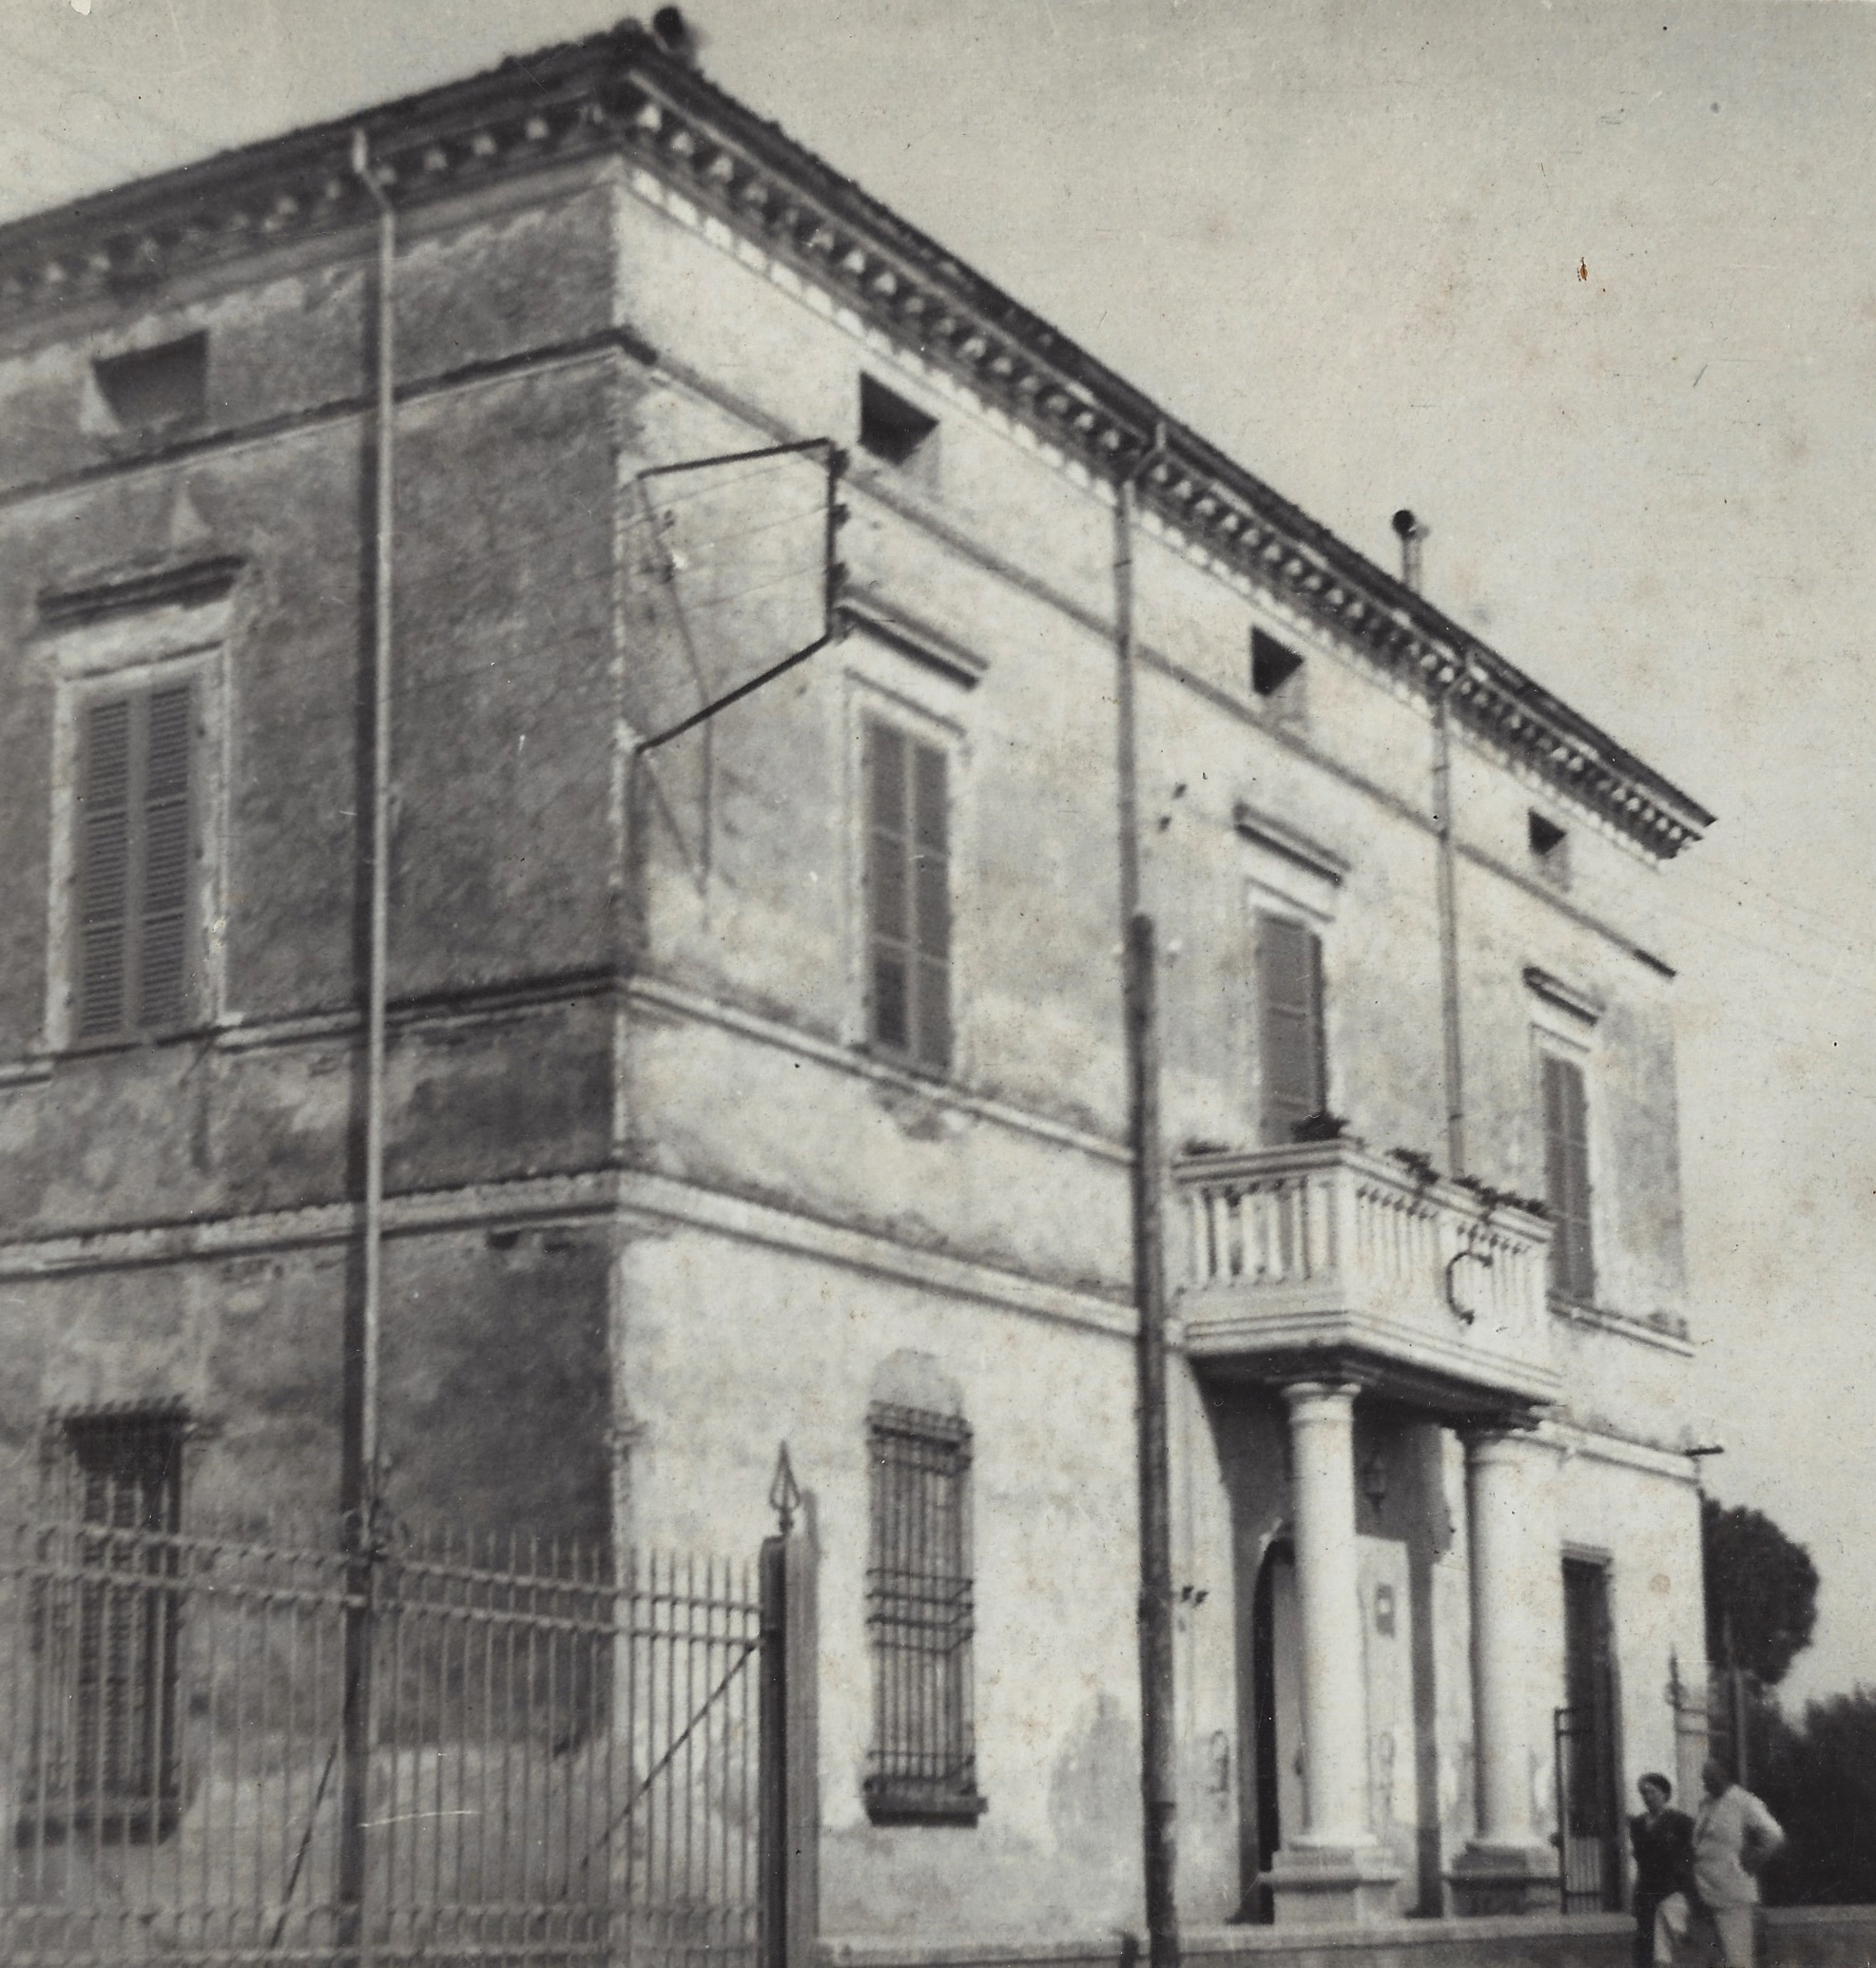
\includegraphics[width=\textwidth]{casamingazzi}
    \caption[Palazzo Mingazzi]{Il \textbf{Palazzo Mingazzi}, in via Reale 97. In basso a destra si può notare Stefano Mingazzi con la moglie Amalia Isani. Alla morte di Amalia, la casa passò all'erede universale di Mingazzi, ovvero l'Istituto dei Ciechi di Bologna. Minguzzi Egisto comprò tutti i terreni tra cui anche il palazzo Mingazzi. Questo edificio non era in buone condizioni perciò Egisto decise di abbatterlo. (ndr) Dalle testimonianze che ho raccolto, all'entrata si poteva vedere subito una ripida ma maestosa scalinata in legno.\label{fig:casamingazzi}}
    %\vspace{-0.3cm}
\end{figure}



































%